\section{Resultat}
todo

\subsection{Parser} 
%TODO
Parsern uppgift är att ta användarens indata och konvertera den till en datastruktur 
som är lättare att hantera internt. Denna datastruktur kallas AST (Abstract Syntax Tree). 
Haskellstandarden definerat upp en grammatik, ett antal regler som definerar hur korrekt Haskellkod ser ut och hur den ska tolkas.

För att parsa indatan använder vi ett bibliotek för att bygga parsers kallat JSParse \citep{jsparse}.
JSParse ger os ett antal funktioner som vi använder för att definera grammatiken och konvetera den till vår interna struktur.

Parsern består av tre parsers, den första är en parser som hittar kommentarer och tar bort dessa. 
Den andra identifierar haskellkod som inte är kontextfri och gör om till kontextfri kod. Den tredje gör om den kontextfria koden till vår AST.

\begin{figure}[H]
    \begin{center}
        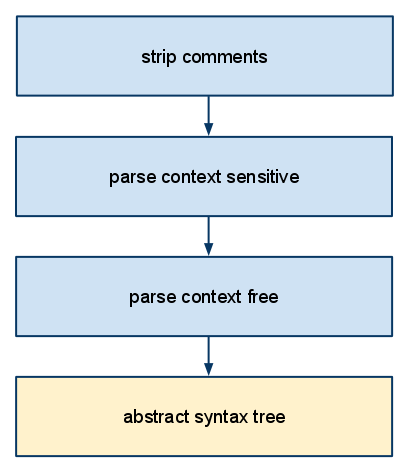
\includegraphics[width=.5\textwidth]{parser_1.png}
        \caption{Parserns olika steg}
    \end{center}
\end{figure}

Det var naturligt att dela upp parsern i tre olika steg. De tre olika stegen är skilda från varandra och vi kunde utveckla och testa dem individuellt.

Nedan följer ett exempel på parserns arbetssätt och de tre olika stegen:
\begin{lstlisting}
-- Kommentar
f x = case x of
    True -> False
    False -> True
\end{lstlisting}

Efter första steget:
\begin{lstlisting}
f x = case x of
    True -> False
    False -> True
\end{lstlisting}

Efter andra steget:
\begin{lstlisting}
f x = case x of {
    True -> False;
    False -> True
}
\end{lstlisting}

Efter det tredje steget har vi en AST.
\begin{lstlisting}
Function("f", Lambda("x", 
    Case(ast.VariableLookup("x"), [
        [PatternConstructor("True"), PatterConstructor("False")],
        [PatternConstructor("False"), PatterConstructor("True")],
    ])
))
\end{lstlisting}

\subsubsection{Steg 1}
Det första steget använder en parser som identifierar och tar bort kommentarer. 
Haskell har två olika kommentarsstiler, enkelradiga börjar med '--' och slutar vid första radbytet och 
nästlade som kan gå över flera rader börjar med '{-' och slutar med '-}'.

\subsubsection{Steg 2}
Det andra steget delar upp koden i dess ord och symboler samtidigt som den dekoreras med indenteringsnivåer enligt en algoritm 
som är specifierad i Haskellstandarden. Därefter användads en annan algoritm från standarden för att sätta in måsvingar och semikolon på rätt platser. 
När de två algoritmerna är klara sätts koden ihop igen och skickas vidare till nästa steg.

En regel är att ett inre block inte får vara mindre indenterat än det omslutande blocket, exempelivs:
\begin{lstlisting}
case x of
    True -> ...
\end{lstlisting}
Här är \emph{True -> ...} ett inre block till \emph{case} och mer indenterat.

Ett annat exempel är:
\begin{lstlisting}
let x = 5 in x
\end{lstlisting}
Den korrekta översättningen är:
\begin{lstlisting}
let { x = 5 } in x
\end{lstlisting}
För att översätta detta korrekt kommer parsern ihåg den aktuella nästlingsnivån av "let"-uttryck och var deras repsektive "in"-uttryck befinner sig. 
Den avslutande måsvingen sätts in där ett matchande "in"-uttryck påträffas.

Ett exempel som inte översätts korrekt:
\begin{lstlisting}
[x | let x = 2]
\end{lstlisting}
Den korrekta översättningen är:
\begin{lstlisting}
[x | let { x = 2 }]
\end{lstlisting}
Men det blir:
\begin{lstlisting}
[ x | let { x = 2 ] }
\end{lstlisting}
Anledningen är att endast nästlingen av \emph{let} och \emph{in} sparas, men här finns inget \emph{in}.
För att lösa felet måste man hålla reda på antalet paranteser, måsvingar, hakparanteser och komman efter ett let-uttryck och när en symbol som gör det ogiltligt 
med en avslutande måsvinge påträffas sätts måsvingen in precis innan symbolen.

\subsubsection{Steg 3}
Det tredje steget är en parser för hela den kontextfria varianten av Haskell som den är definerad i standarden. 
Samtidigt som koden tolkas byggs en AST upp. Parsern består av en liten parser för varje grammatisk regel som är definerad i Haskellstandarden 
dessa parsers kombineras ihop för att bilda den slutgiltliga parsern. Det resulterar i ett träd av parsers, en parser för hela programmet som har flera mindre parsers under sig.

Exempel:
Definitionen i Haskellstandarden:
\begin{lstlisting}
rhs -> exp [where decls]
     | gdrhs [where decls]
gdrhs -> gd = exp [gdrhs]
\end{lstlisting}
Dess respektive parsers:
\begin{lstlisting}
var gdrhs = gdrhs_action(
    repeat1(gdrhs_fix_list_action(sequence(ws(gd), 
                expectws('='), ws(exp)))));´

var rhs = choice(
    decl_rhs_action(sequence(expect(ws('=')), ws(exp), 
         optional(sequence(expect(ws("where")), ws(decls))))),
     sequence(ws(gdrhs), optional(sequence(expect(ws("where")), 
         ws(decls))))
);
\end{lstlisting}

\subsubsection{JSParse}
Vi använder en modifierad version av JSParse där vi har korrigerat två fel och lagt till fler parsers. Felen vi korrigerade var i butnot-parsern och i choice-parserns cachefunktion. 
Choice-parsern cachade resultat från parsers som misslyckades och det cachade resultatet användes i senare parsers, 
vi löste det med en stackbaserad cache där cachen för en parser som misslyckas raderas.

Parsers som vi har lagt till:
\begin{enumerate}
    \item{\emph{repeatn}: en parser som upprepar en parser minst \emph{n} antal gånger}
    \item{\emph{expectws}: en parser som tillåter blanksteg och inte retunerar någon ast, är en kombination av JSParse inbyggda parsers \emph{expect} och \empth{whitespace}}
\end{enumerate}

\subsection{Abstrakt syntaxträd} 
%TODO

\subsection{Typcheckare} 
%TODO

\subsection{Interpretator}

Interpretatorn är...

Non strict, att evaluera ett uttryck resulterar i en thunk. En thunk kan tvingas till ett Weak Head Normal Form (WHNF) [referens] under flera olika omständigheter.
~ Pattern Matchning
~ funktionsapplikation
~ Argument till primitiv funktion

~ dereferencing a pointer returns a whnf.

~ Env är en samling HeapPtr.


~ konvetionellt desugar efter typchecking för att få bra felmedelanden vid typfel
Vi desugar under runtime, för att få bra möjligheter till interaktion.

~ Desugaring do

~ Desugaring list comprehension

~ Desugaring arithmetic sequence

~ Regler för evaluering (retunerar en WHNF eller closure)



\subsection{HIJi}
HIJi, Haskell in Javascript Interactive, är den del av projektet som användaren tydligast kommer märka av eftersom det är fasaden in i programmet.
HIJi erbjuder användaren ett GHCi-liknande användargränssnitt direkt i webläsaren. 
HIJi tar input genom att användaren skriver funktioner och uttryck i HIJi. När användaren klickar på retur tolkas inputen av parsern och bygger upp det abstrakta syntaxträdet. Därefter evalueras uttrycket utav interpretern.
Det går även att ladda moduler till HIJi. Det gör man genom att skriva :l \emph{namn-på-modul}. Man får då tillgång till alla de funktioner som är skrivna i den modulen. HIJi har även en förladdad modul, Prelude, som innehåller en delmängd av de funktioner som finns i GHCs motsvarighet.  

Den indata som användaren skriver till HIJi sparas i ett objekt för att hantera historiken. Man bläddrar i historiken med piltangenterna Upp och Ner. Hela historik-objektet sparas även i en kaka som ett JSON-objekt. Av detta skäl är det möjligt att få tillgång till historiken när man startar en ny session av webbläsaren. Historiken laddas in när HIJi startar.

HIJi är skapat för att likna GHCi i så stor utsträckning som möjligt.
Genom att efterlikna GHCi kommer användare känna igen sig när de tar steget från HIJi till GHCi. Det blir för dem ett naturligt steg och kortar inlärningströskeln. Även för haskellprogrammerare som är väl införstådda i GHCi's möjligheter blir det lättare att använda sig utav HIJi, de behöver inte fundera hur verktyget ska användas.
Dock finns det vissa nackdelar med ett terminalbaserat användargränssnitt. Terminalbaserade användargränssnitt anses inte vara lika enkelt och intuitivt att förstå som ett grafiskt användargränssnitt. 

\begin{figure}[H]
    \begin{center}
        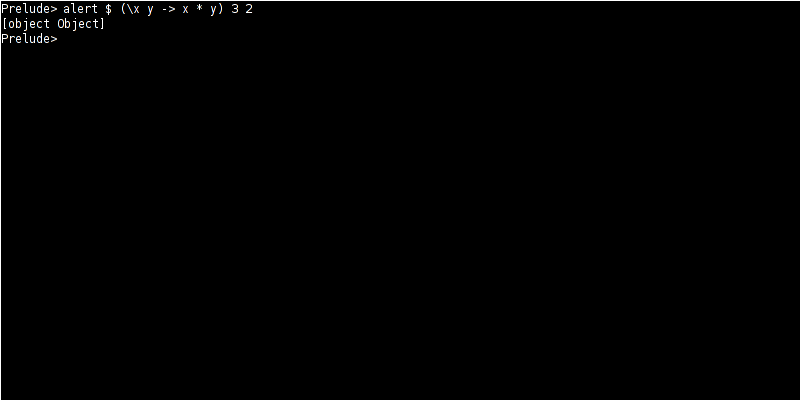
\includegraphics[width=1\textwidth]{hiji_screen3.png}
        \caption{HIJi användargränssnitt}
    \end{center}
\end{figure}

Figur 2 visar hur HIJi ser ut för användaren. De första raderna visar precis som i GHCi vilka moduler som för närvarande är laddade. I detta exemplet är den förladdade modulen Prelude laddad. Därefter följer en prompt där användaren fritt kan skriva in egna funktioner. I figuren har användaren skrivit en lambda-funktion.

Fördelen med HIJi framför GHCi är att användaren ej behöver ladda ner den stora GHC-kompilatorn på sin personliga dator för att testa enkla Haskelluttryck direkt i webbläsaren. Den åtgångna tiden från  att man vill testa Haskell till dess att man faktiskt sitter med det framför sig kortas. 
Nackdelar gentemot GHCI är att HIJi är en nedbandat version utav GHCi. HIJi kan bara evaluera enklare uttryck. Det finns i dagsläget inga möjligheter att ladda upp hela Haskell-filer för att köra dem. Att som i GHCi på ett enkelt sätt kolla upp  typen av en funktion stöds ej.


